\section{Contraintes}
Réalisation d'un effet \emph{fisheye} en flex. L'idée est d'appliquer l'effet sur les conteneur présents dans le conteneur appliquant le layout \emph{fisheye}, sous la forme d'une grille dont les éléments grandisse en fonction de la proximité avec la souris.

Dans l'idéal, l'effet produit doit minimiser l'espace entre les conteneurs.

\section{Analyse \& implémentation}

Nous avons fait le choix de créer un layout \emph{fisheye} assurant les traitements nécessaire à la réalisation de l'effet. Pour cela, nous avons utilisé le namespace spark permettant de dissocier le container du layout. Il sera ainsi possible d'associer le layout personnalisé à n'importe quel container spark. Le layout appliquera l'effet sur tous les container dont le container parent est celui sur lequel est appliqué le layout \emph{fisheye}.

Pour la réalisation de ce layout, nous avons eu deux approches qui sont détaillées ci-après.

\subsection{Approche globale}
Cette approche suppose qu'il est possible, en connaissant la position de la souris et la position d'un bloc, de le placer et le dimensionner exactement sur la grille. Les caractéristiques du bloc ne dépendent donc pas du placement des autres blocs voisins.

Le layout peut être paramétré de la manière suivante :

\begin{description}
  \item[maxSize] Taille maximum de l'élément dans la grille,
  \item[minSize] Taille minimum de l'élément dans la grille,
  \item[spread] Propagation de l'agrandissement autour de la souris,
\end{description}

Ainsi le layout va initialiser les éléments sur une grille de la manière suivante :
\begin{figure}[H]
  \centering
  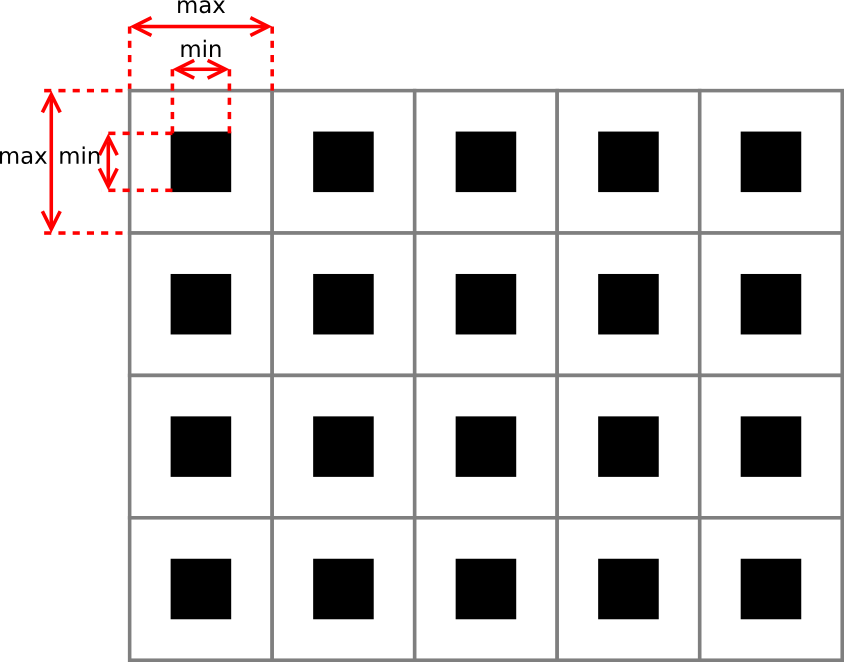
\includegraphics[width=\textwidth]{../resources/illustrations/grob_app_init}
  \caption{Initialisation des éléments avec l'approche globale.}
\end{figure}

Un \emph{eventlistener} capture les mouvements de la souris dans le but de mettre à jour chaque \emph{container} de la grille.

\begin{figure}[H]
  \centering
  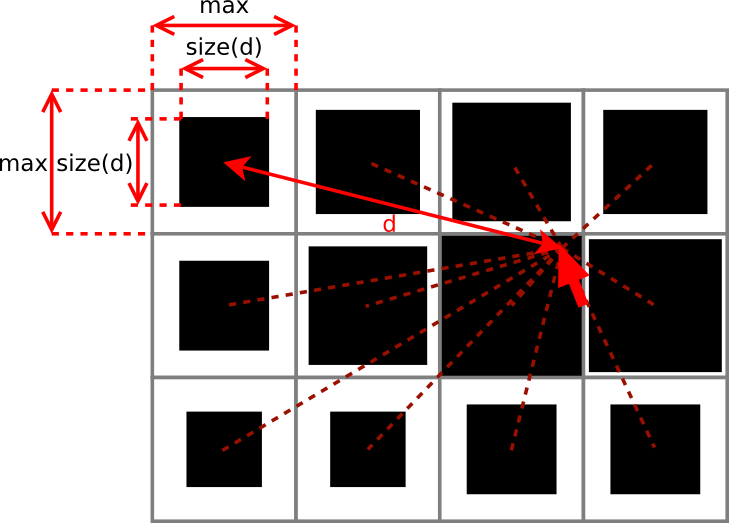
\includegraphics[width=\textwidth]{../resources/illustrations/grob_app_mouse}
  \caption{Mise à jours des éléments avec l'approche globale.}
\end{figure}

La taille des éléments sont mis à jours en fonction de la distance entre le centre du block et le pointeur de la souris. Dans tous les cas les éléments restent alignés dans la grille par le fait que les centres des objets ne sont pas déplacés.

Après implémentation et test avec des containers colorés en noir, on obtient ceci :

\begin{figure}[H]
  \centering
  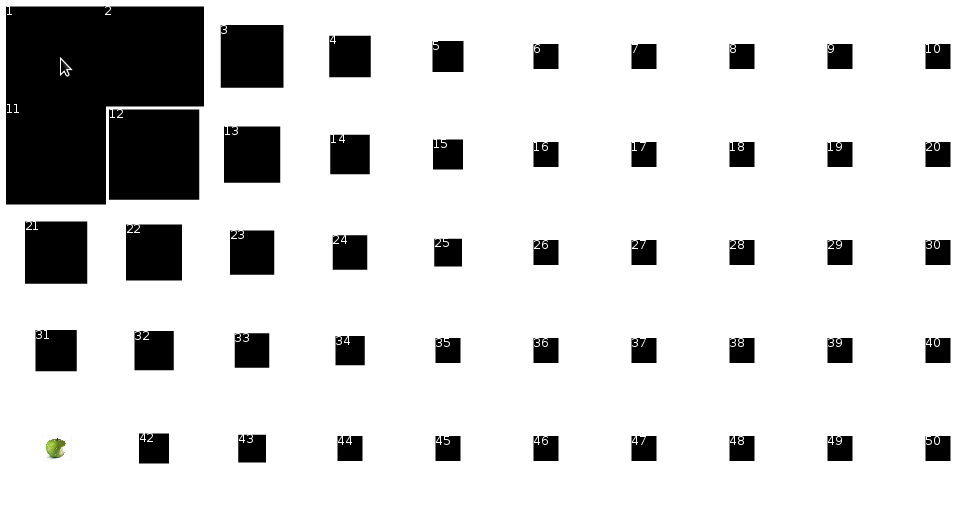
\includegraphics[width=\textwidth]{../resources/illustrations/c1}
  \caption{Premier aperçu.}
\end{figure}

\begin{figure}[H]
  \centering
  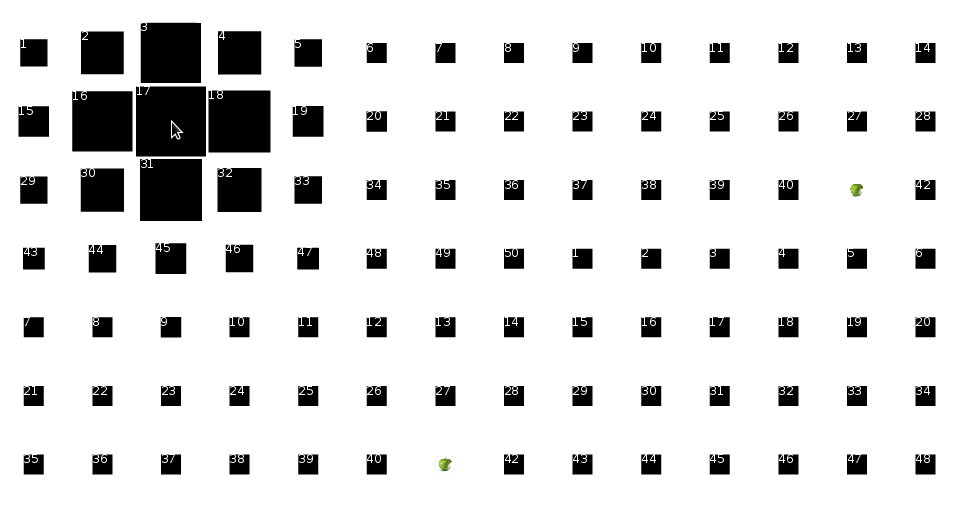
\includegraphics[width=\textwidth]{../resources/illustrations/c2}
  \caption{Second aperçu.}
\end{figure}

L'avantage de ce type d'approche est d'arriver rapidement à un résultat fluide et  satisfaisant. Le principal problème réside dans l'espacement entre les éléments de la grille. Un solution\footnote{Solution non implémentée.} pourrait consister en la mise en place d'une attraction des éléments vers le pointeur de la souris : plus les éléments sont éloignés, plus ils sont attirés vers la souris. On obtiendrait quelque chose comme suit :

\begin{figure}[H]
  \centering
  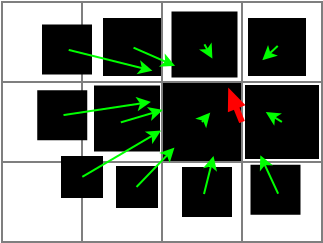
\includegraphics[width=\textwidth]{../resources/illustrations/grob_app_evo}
  \caption{Évolution permettant de réduire l'espace entre les éléments de la grille.}
\end{figure}

\subsection{Approche propagée}

Cette approche est différente. Les dimensions et la position de chaque élément dépend des autre, et sont affectés au travers d'un parcours séquentiel.

Ici les éléments sont initialisé par une valeur moyenne ainsi qu'une marge entre les éléments.

\begin{figure}[H]
  \centering
  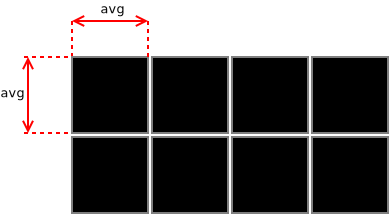
\includegraphics[width=\textwidth]{../resources/illustrations/seq_app_init}
  \caption{Initialisation par la méthode propagée.}
\end{figure}

Lors d'un mouvement de souris, le parcours débute par l'élément le plus proche de la souris, affecte les positions et tailles des éléments sur la ligne, puis le traitement est effectué de manière récursive pour chaque autre ligne.

\begin{figure}[H]
  \centering
  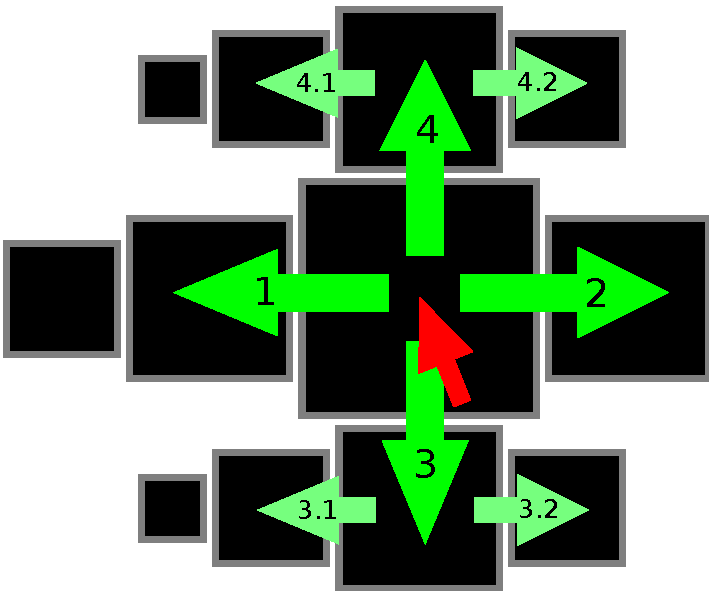
\includegraphics[width=\textwidth]{../resources/illustrations/seq_app_mouse}
  \caption{Évolution permettant de réduire l'espace entre les éléments de la grille.}
\end{figure}

Ce rendu a été réalisé mais n'est pas exploitable pour deux raisons :

\begin{itemize}
  \item pas de fluidité lors du passage de la souris entre deux éléments,
  \item disposition peu ergonomique.
\end{itemize}

Dans le but d'améliorer le second point, la disposition des éléments des ligne pourrait être améliorer\footnote{Amélioration non implémentée.}. La première évolution propose de contraindre la distribution des éléments de chaque ligne en se basant sur la grille générée au fur et à mesure du parcours. La seconde évolution fonctionne de la même manière, mais déplace les éléments dans le coin le plus proche de l'élément sélectionné.

\begin{minipage}[H]{.5\linewidth}
\begin{figure}[H]
  \centering
  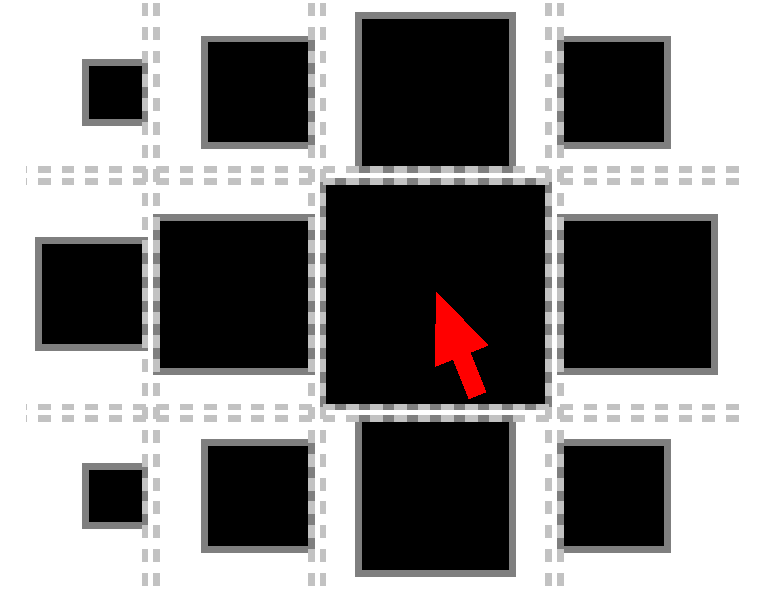
\includegraphics[width=\textwidth]{../resources/illustrations/seq_app_mouse_v2}
  \caption{Première évolution permettant un meilleur affichage de la grille.}
\end{figure}
\end{minipage}
\begin{minipage}[H]{.5\linewidth}
\begin{figure}[H]
  \centering
  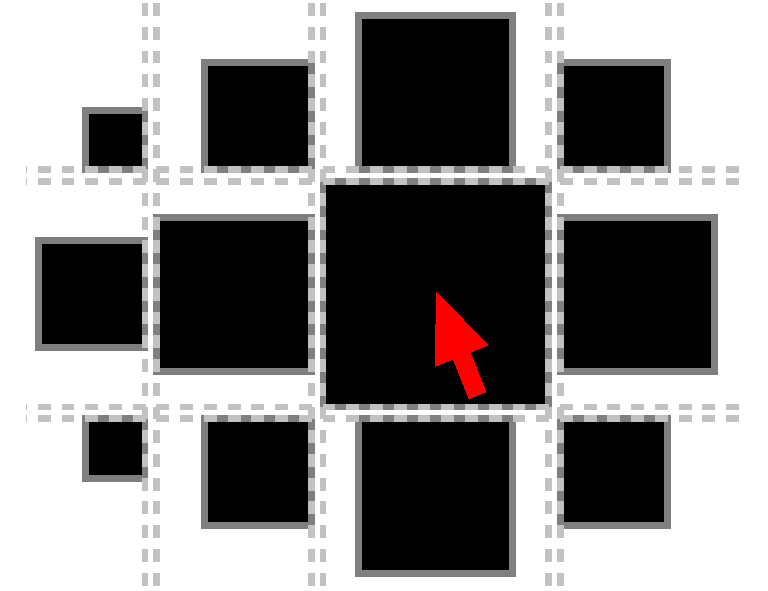
\includegraphics[width=\textwidth]{../resources/illustrations/seq_app_mouse_v3}
  \caption{Seconde évolution permettant un meilleur affichage de la grille.}
\end{figure}
\end{minipage}

\subsection{Approche mathématique}

La dernière approche est une approche mathématique. L'idée est de
considérer l'ensemble des éléments comme un tableau d'éléments puis de
jouer sur la largeur des colonnes et la hauteur des lignes.

\begin{figure}[H]
  \centering
  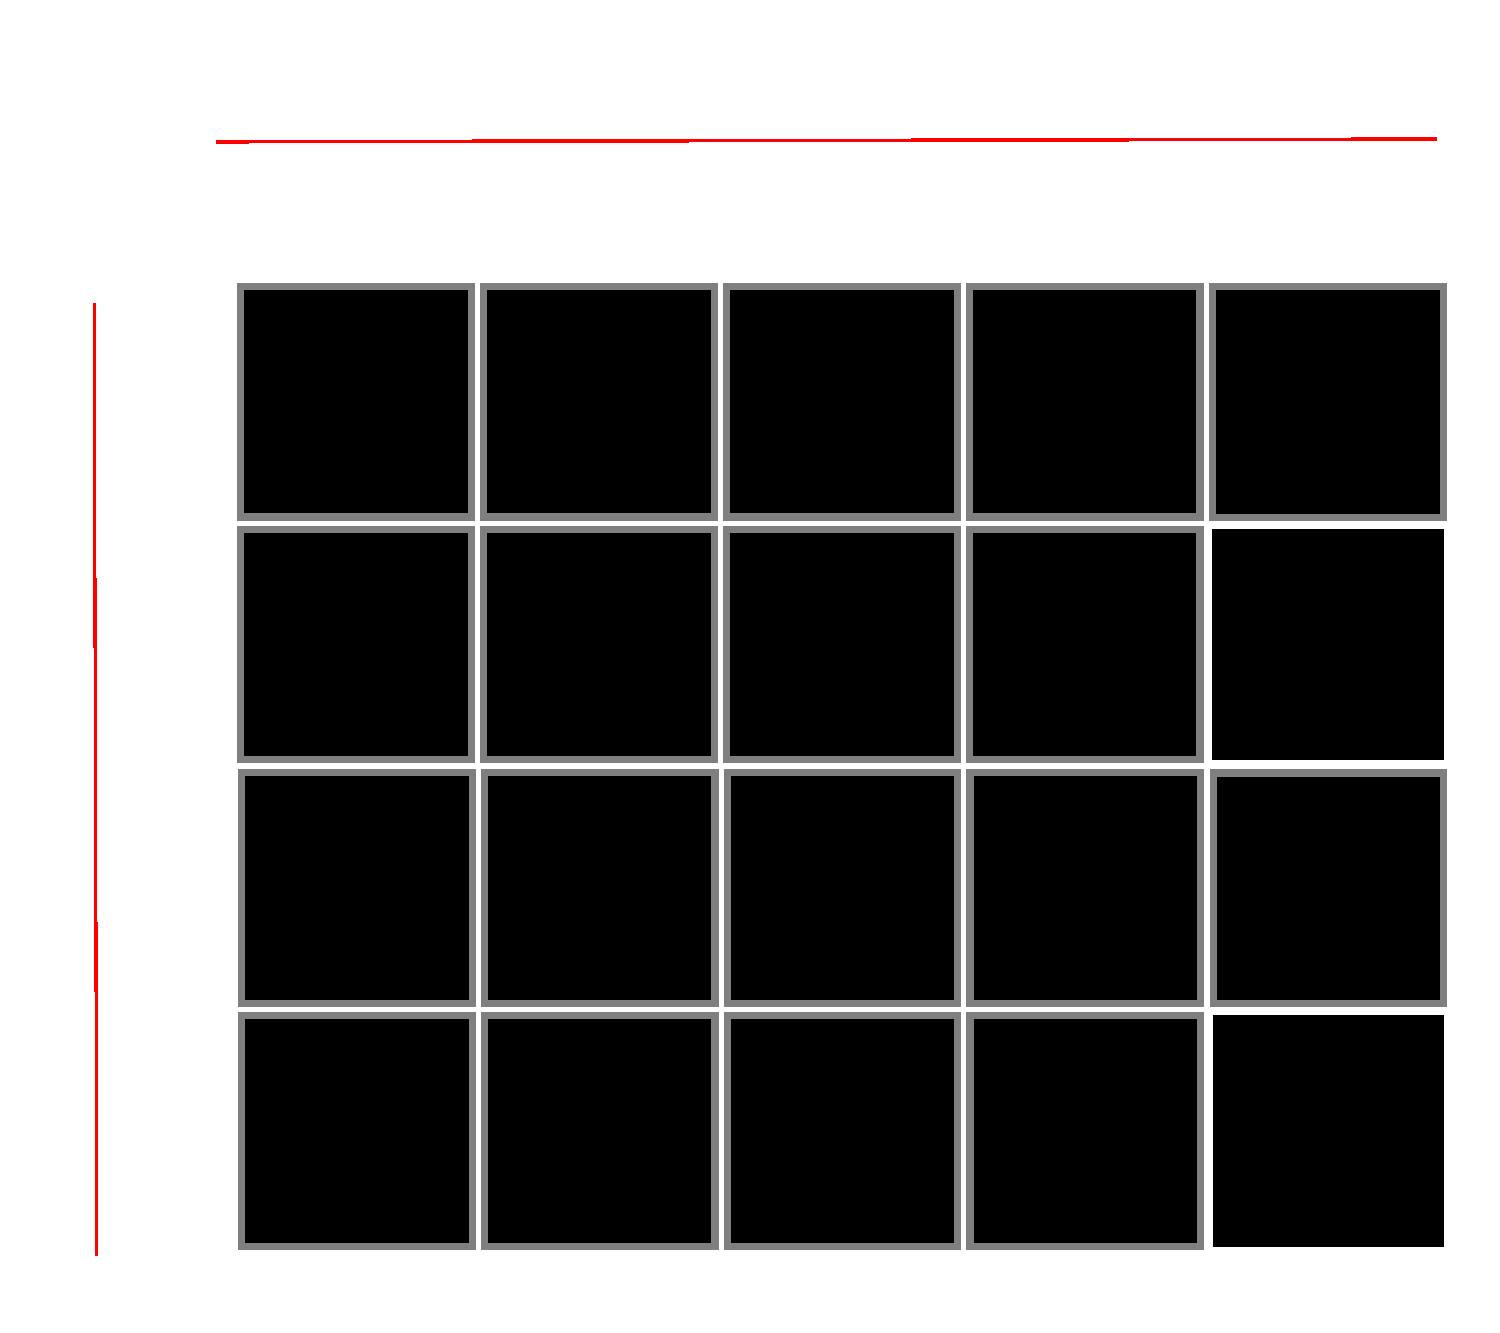
\includegraphics[width=0.7\textwidth]{../resources/illustrations/js_1}
  \caption{Grille d'éléments sans présence de la souris}
  \label{fig:js_1}
\end{figure}

La figure \ref{fig:js_1} ci-dessus représente l'état du tableau en
l'absence de la souris. Dans ce cas, la largeur et la hauteur des
cellules est représentées par une fonction constante. La figure
\ref{fig:js_2} montre comment la largeur et la hauteur des cellules
sont modifiées par la présence de la souris. La nouvelle taille des
cellules est calculée grâce à deux fonctions gaussiennes indépendante,
une pour la largeur et une autre pour la hauteur.  

\begin{figure}[H]
  \centering
  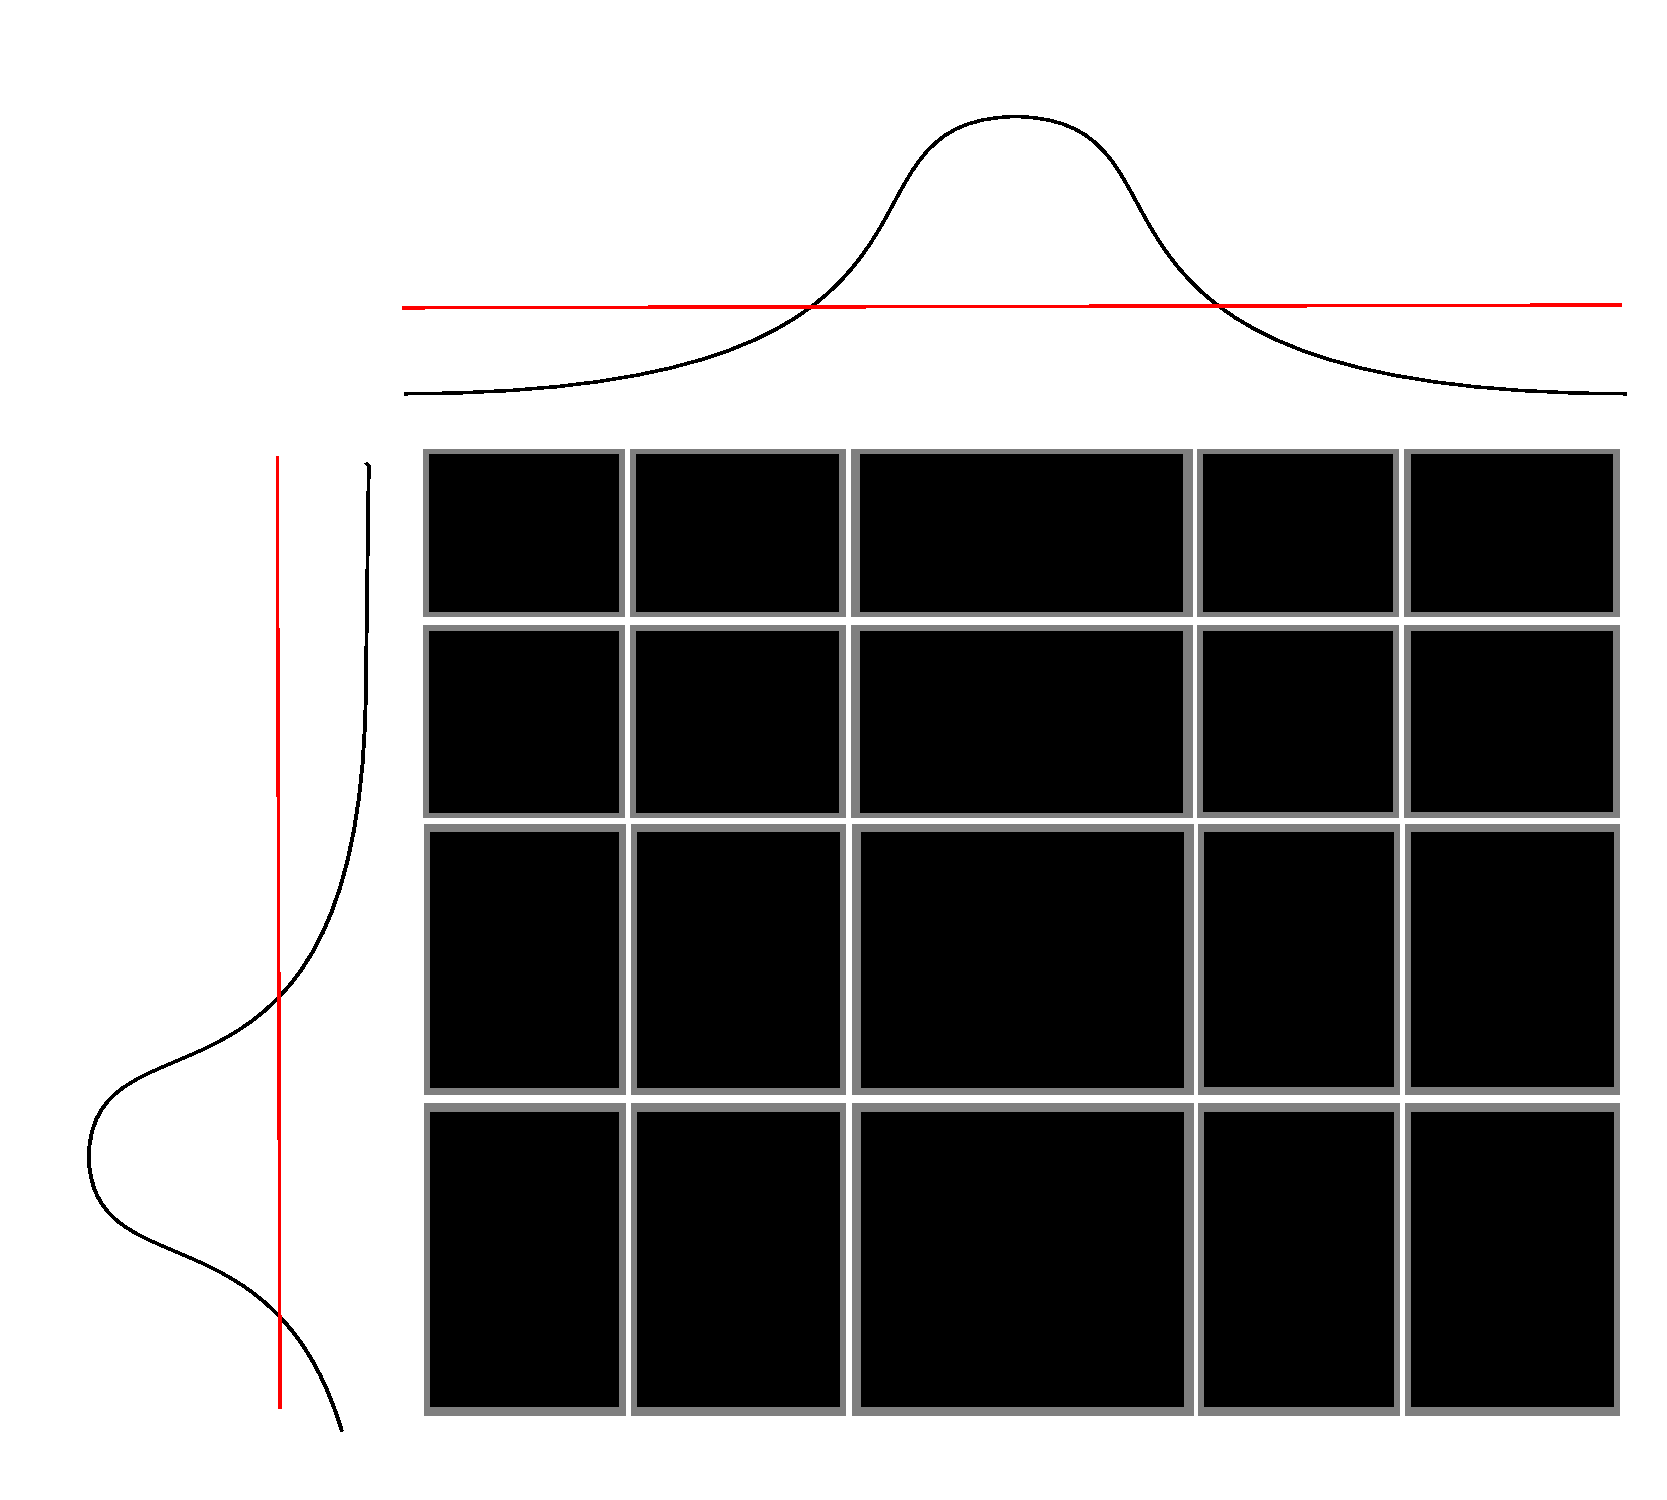
\includegraphics[width=0.7\textwidth]{../resources/illustrations/js_2}
  \caption{Grille d'éléments modifié par la présence de la souris}
\end{figure}

Ces fonctions sont 
$\frac{facteur\_grossissement}{{dist/attenuation}^{2}+0.5}-facteur\_grossissement$

\begin{figure}[H]
  \centering
  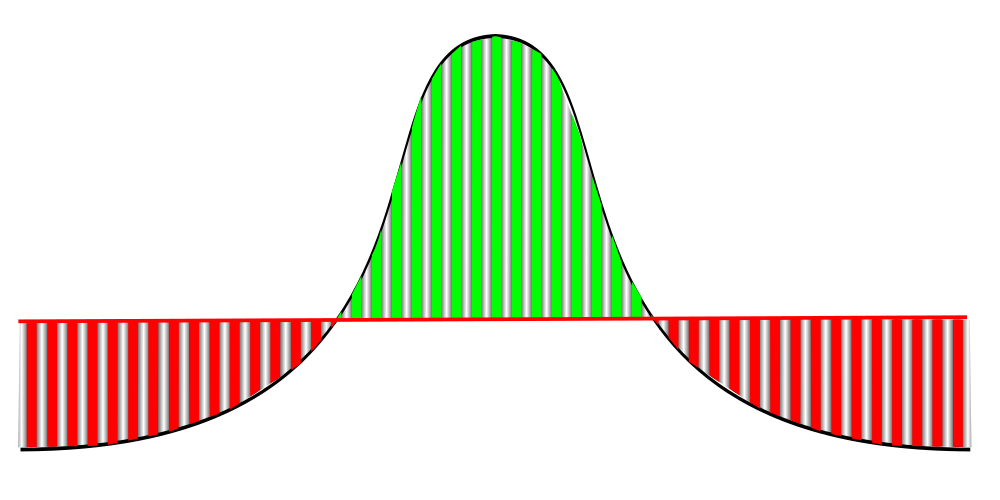
\includegraphics[width=0.7\textwidth]{../resources/illustrations/js_3}
  \caption{Courbe de déformation}
\end{figure}

\begin{figure}[H]
  \centering
  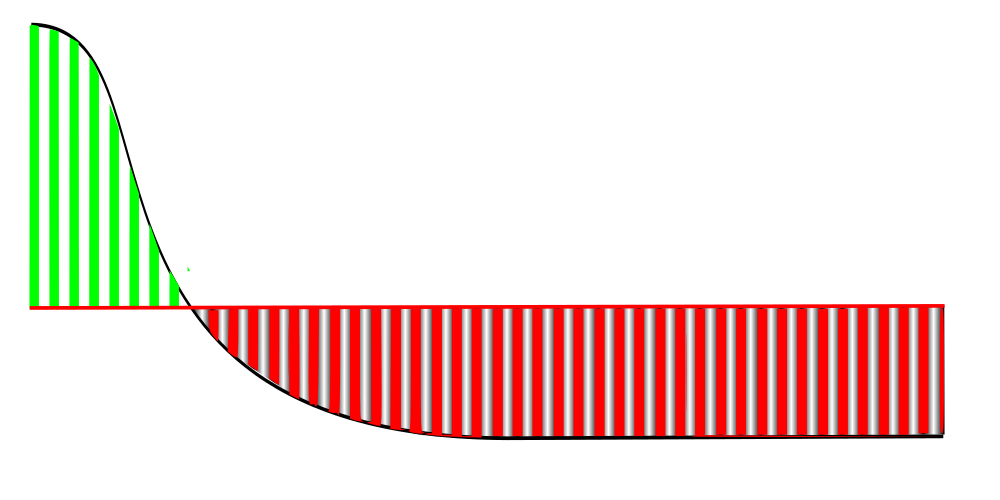
\includegraphics[width=0.7\textwidth]{../resources/illustrations/js_4}
  \caption{Courbe de déformation}
\end{figure}

\begin{figure}[H]
  \centering
  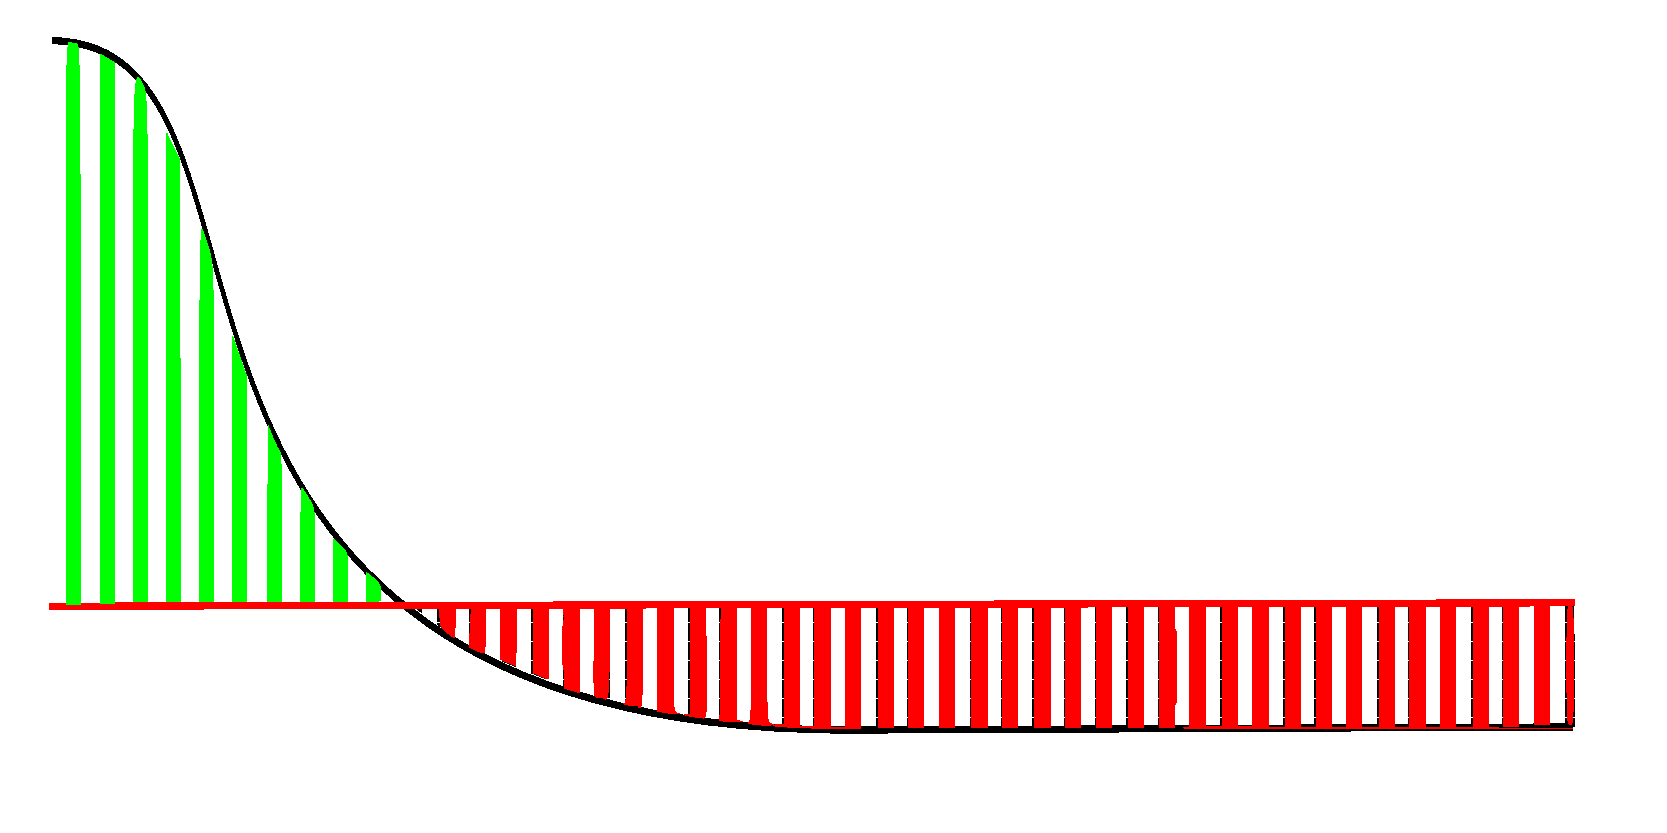
\includegraphics[width=0.7\textwidth]{../resources/illustrations/js_5}
  \caption{Courbe de déformation}
\end{figure}

\section{Environnement de travail}

Dans le but de réellement découvrir flex, nous avons fait le choix de ne pas utiliser Flash Builder\footnote{En réalité nous n'avions pas le choix, aucune version étant disponible sous GNU/Linux.}. Le développement a donc été effectué via un éditeur de texte avec complétion syntaxique pour \emph{mxml} et \emph{actionscript}. La compilation a été exécutée en ligne de commande.